\documentclass[aspectratio=169]{beamer}

\usetheme{Madrid}
\usecolortheme{default}
\setbeamertemplate{navigation symbols}{}

\usepackage[utf8]{inputenc}
\usepackage[T1]{fontenc}
\usepackage{graphicx}
\usepackage{booktabs}
\usepackage{hyperref}

\title[StreamCab]{StreamCab: Real-Time Taxi Fare Intelligence}
\subtitle{Final Project Presentation}
\author{Your Name \\ Group Member 1, Group Member 2, Group Member 3}
\institute{Course Name / Department}
\date{\today}

\begin{document}

\begin{frame}
  \titlepage
\end{frame}

\begin{frame}{Presentation Plan (12 min + 3 min Q\&A)}
\begin{itemize}
  \item Overview: problem statement and architecture
  \item Data: source, collection, schema/metadata
  \item Process: end-to-end processing inputs and outputs
  \item Results: dashboard and analytics outcomes
  \item Key takeaways: what was easy and difficult
\end{itemize}
\end{frame}

\begin{frame}{1. Overview: Problem Statement}
\textbf{Problem:}
\begin{itemize}
  \item Taxi demand and pricing patterns change quickly by time and location.
  \item Drivers and operators need near real-time signals for fare and zone activity.
\end{itemize}

\textbf{Goal:}
\begin{itemize}
  \item Build an end-to-end streaming analytics pipeline that:
  \begin{itemize}
    \item ingests NYC taxi trip events,
    \item computes rolling traffic aggregates,
    \item predicts short-term average fare by pickup zone,
    \item serves insights in an interactive dashboard.
  \end{itemize}
\end{itemize}
\end{frame}

\begin{frame}{1. Overview: System Architecture}
\begin{center}
  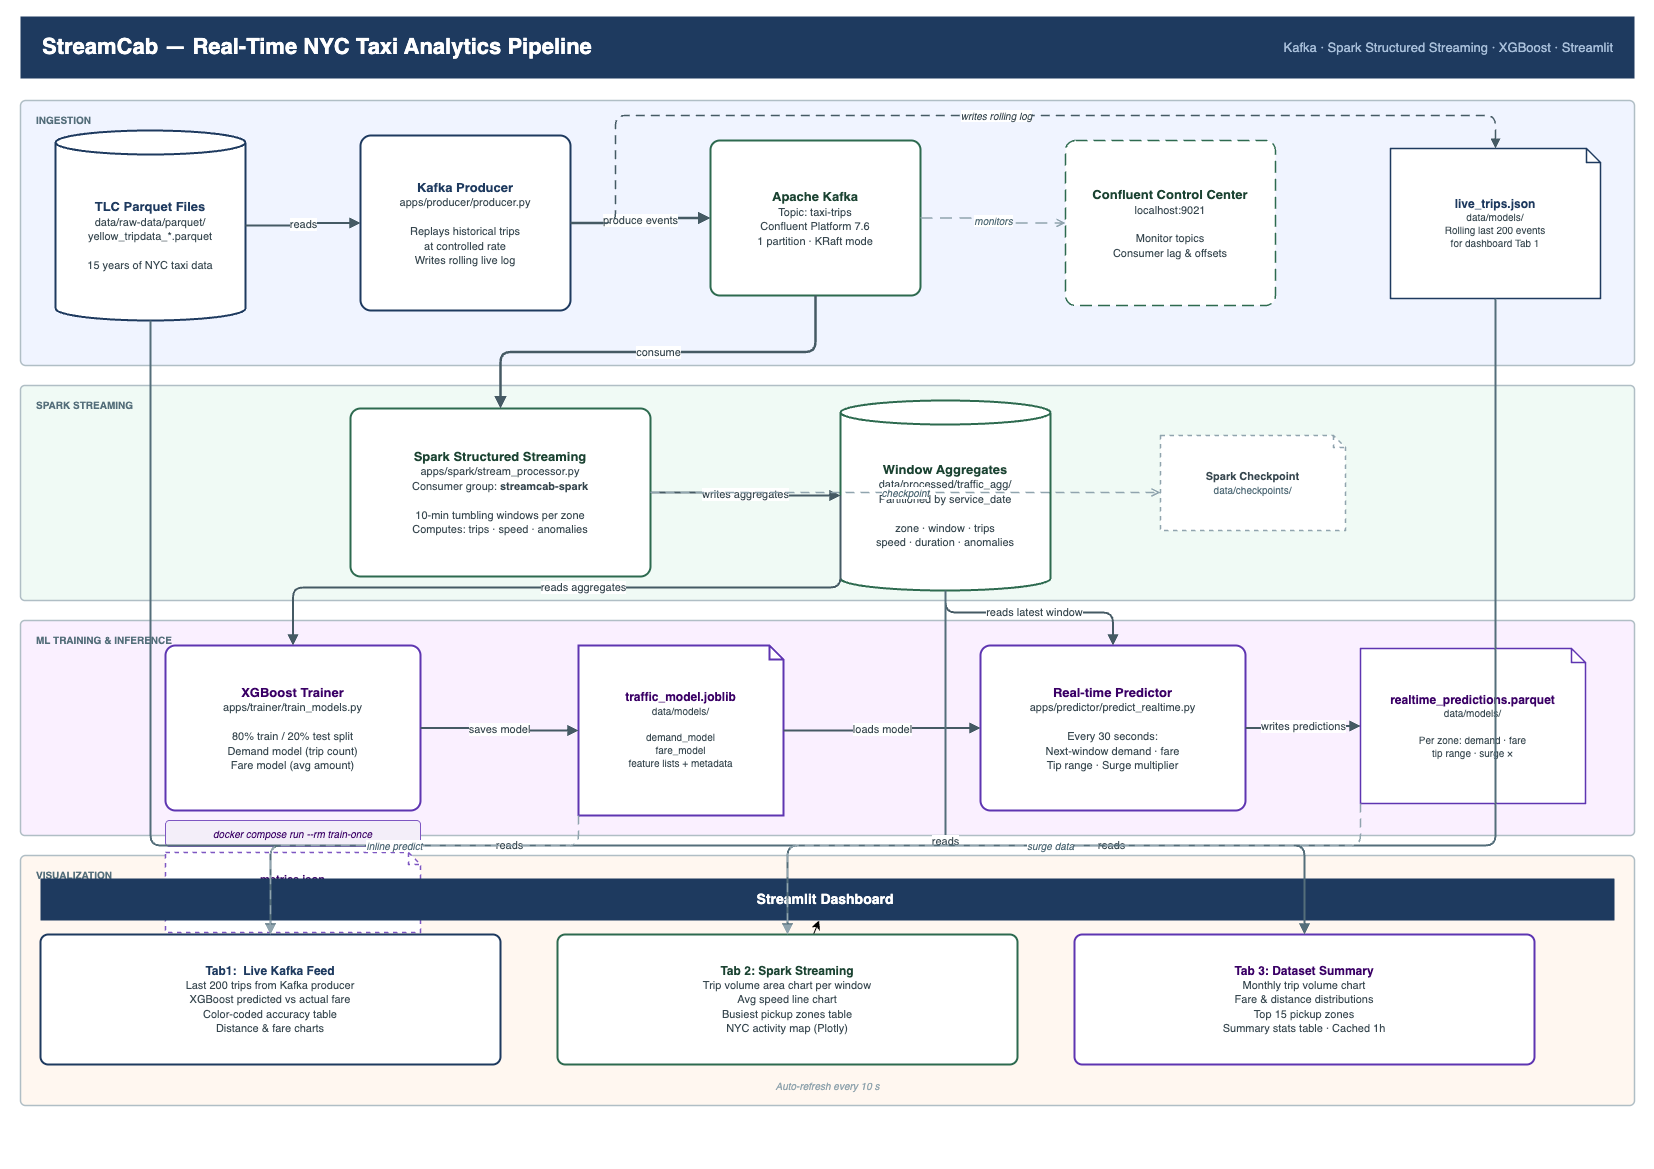
\includegraphics[width=0.95\linewidth]{../assets/architecture.png}
\end{center}
\vspace{0.3em}
\small
Pipeline summary: \texttt{Parquet -> Kafka -> Spark -> Postgres -> Predictor -> Dashboard}
\end{frame}

\begin{frame}{Architecture Components}
\begin{itemize}
  \item \textbf{Producer + Kafka:} replays parquet trips as event stream.
  \item \textbf{Spark Structured Streaming:} cleans and aggregates by zone/window.
  \item \textbf{Postgres:} stores live trips, aggregate traffic, and predictions.
  \item \textbf{Trainer (XGBoost):} trains fare model from historical data.
  \item \textbf{Predictor:} periodic inference on latest per-zone aggregates.
  \item \textbf{Streamlit Dashboard:} live KPIs, rankings, map, and predictions.
\end{itemize}
\end{frame}

\begin{frame}{2. Data: Source and Collection}
\textbf{Primary source:}
\begin{itemize}
  \item NYC TLC yellow taxi trip records (public monthly parquet files).
\end{itemize}

\textbf{Collection workflow:}
\begin{itemize}
  \item Download selected month range with project script.
  \item Store raw files under local parquet directory.
  \item Replay rows as Kafka events for streaming simulation.
\end{itemize}

\textbf{Reference data:}
\begin{itemize}
  \item TLC zone centroids file for geospatial zone mapping.
\end{itemize}
\end{frame}

\begin{frame}{2. Data: Schema and Metadata}
\small
\textbf{Event-level fields (example):}
\begin{itemize}
  \item pickup\_datetime, dropoff\_datetime
  \item passenger\_count, trip\_distance
  \item pu\_location\_id, do\_location\_id
  \item total\_amount, emitted\_at
\end{itemize}

\textbf{Aggregated output (windowed):}
\begin{itemize}
  \item window\_start/window\_end, pu\_location\_id, trip\_count
  \item avg\_speed\_mph, avg\_duration\_min, avg\_trip\_distance
  \item avg\_total\_amount, anomaly\_count
\end{itemize}

\textbf{Prediction output:}
\begin{itemize}
  \item predicted\_avg\_fare, predicted\_tip\_low/high, surge\_multiplier
\end{itemize}
\end{frame}

\begin{frame}{3. Process: End-to-End Method}
\begin{enumerate}
  \item Ingest historical parquet data and replay into Kafka.
  \item Consume stream and run quality filters (distance, speed, duration bounds).
  \item Aggregate by pickup zone and sliding windows in Spark.
  \item Upsert aggregates into Postgres for stable serving.
  \item Train XGBoost fare model (continued training with batch updates).
  \item Score latest per-zone aggregates and write predictions.
  \item Render live dashboard with KPIs, rankings, and map views.
\end{enumerate}
\end{frame}

\begin{frame}{3. Inputs and Outputs}
\textbf{Inputs}
\begin{itemize}
  \item Historical parquet trip files
  \item Zone centroid reference CSV
\end{itemize}

\textbf{Intermediate outputs}
\begin{itemize}
  \item Kafka event stream
  \item Postgres tables: \texttt{live\_trips}, \texttt{traffic\_agg}
\end{itemize}

\textbf{Final outputs}
\begin{itemize}
  \item Trained model: \texttt{traffic\_model.joblib}
  \item Metrics: \texttt{metrics.json}
  \item Dashboard + prediction table: \texttt{predictions}
\end{itemize}
\end{frame}

\begin{frame}{Tools Brief (if not covered in class)}
\textbf{Apache Kafka}
\begin{itemize}
  \item Distributed event streaming platform for decoupled producers/consumers.
\end{itemize}
\textbf{Spark Structured Streaming}
\begin{itemize}
  \item Micro-batch stream processing using DataFrame API and watermarks/windows.
\end{itemize}
\textbf{JDBC / Psycopg}
\begin{itemize}
  \item JDBC: Spark connector for SQL sinks.
  \item Psycopg: Python Postgres driver for predictor and consumer services.
\end{itemize}
\end{frame}

\begin{frame}{4. Results: Dashboard and Analytics}
\begin{itemize}
  \item Live trip ingestion and per-minute throughput
  \item Per-zone fare predictions and surge indicators
  \item Most active zones and map-based situational awareness
\end{itemize}

\vspace{0.4em}
\begin{center}
  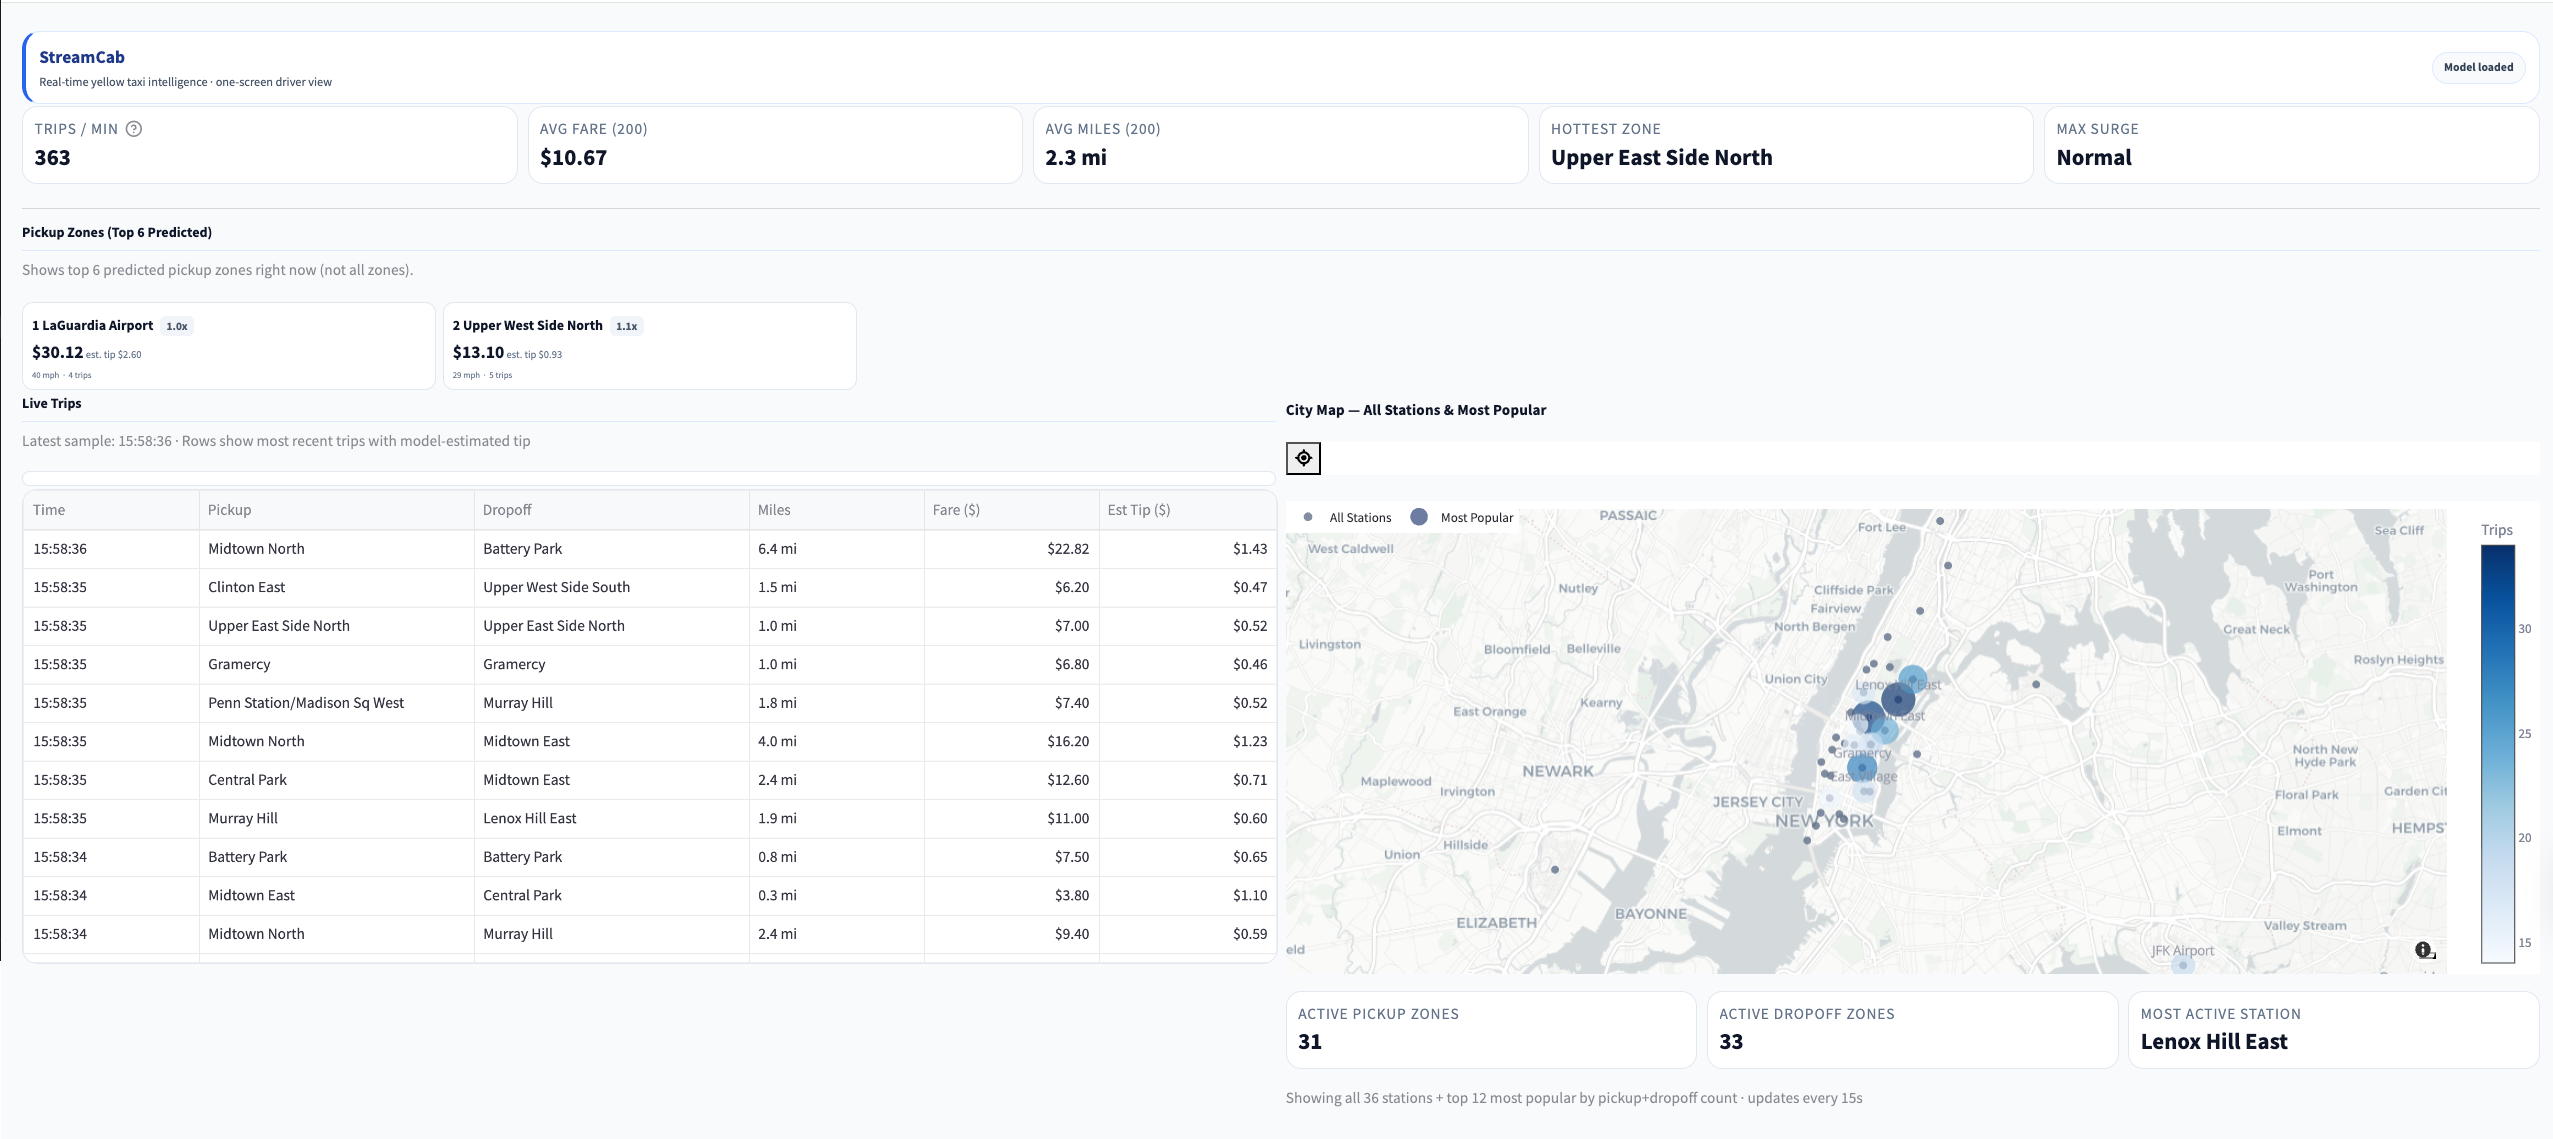
\includegraphics[width=0.82\linewidth]{../assets/app.png}
\end{center}

\vspace{0.5em}
\textbf{Demo assets to include in final slides:}
\begin{itemize}
  \item Dashboard screenshot (current slide) from project assets
  \item Short screen recording or live demo fallback
  \item Model metrics table (baseline vs XGBoost)
\end{itemize}
\end{frame}

\begin{frame}{4. Results: Example Metrics Slide}
\small
\begin{tabular}{lcc}
\toprule
Model & MAE & MAPE (\%) \\
\midrule
Baseline (zone-hour mean) & 1.9891 & 15.43 \\
XGBoost (test) & 0.4851 & 3.42 \\
\bottomrule
\end{tabular}

\vspace{0.8em}
\textbf{Interpretation:}
\begin{itemize}
  \item Significant reduction in absolute and percentage error.
  \item Streaming aggregates provide robust short-horizon features.
\end{itemize}
\end{frame}

\begin{frame}{5. Key Takeaways}
\textbf{What was easier than expected}
\begin{itemize}
  \item Containerized local orchestration with Docker Compose.
  \item Building streaming feature windows with Spark APIs.
\end{itemize}

\textbf{What was difficult}
\begin{itemize}
  \item Memory constraints for large-scale training data.
  \item Exactly-once style behavior across Kafka, Spark, and SQL sink.
  \item Balancing model quality and runtime latency.
\end{itemize}
\end{frame}

\begin{frame}{Reproducibility and Submission Checklist}
\begin{itemize}
  \item GitHub repo includes README walkthrough from input to output.
  \item Public data source link included in README and report.
  \item Final report includes all required sections and references.
  \item Group member names and your name included on both deliverables.
\end{itemize}
\end{frame}

\begin{frame}{Q\&A}
\centering
\Large Thank you.
\end{frame}

\end{document}
